\section{Tests}
Tests that we run on both the two services aimed at verifying their correct behavior - i.e., that the two services were actually confgiured correctly so to be exploited as desired by non-malicious users - and that their setup does not hold a negative impact on the policy implemented in the previous assignment - i.e., the services can be only exploited by authenticated users under certain already mentioned conditions.

\subsection{Testing the VPN}
The \textbf{OpenVPN} service implemented on the \textbf{Main firewall} must be exploited only by an \textit{authenticated user} - that is, a user who owns \textit{three distinct credentials} in order to prove its identity and correctly gain access to the service. These three credentials are: the \textbf{.ovpn} file provided by the \textbf{OPNSense} portal correctly specifying the \textbf{valid cryptographic parameters} to authenticate the user on the \textbf{OpenVPN server}. This file holds the parameters that we previously showed, like port number, authentication type and the cryptographic functions to be arranged during the handshake between client and server, as pictured in \textbf{figure 7}.

\begin{figure}[!htb]
\centering
\begin{minipage}{.33\textwidth}
  \centering
  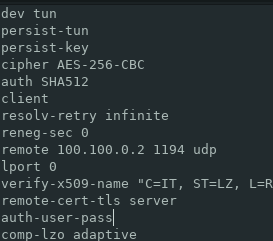
\includegraphics[width=1\textwidth]{ovpnParams.png}
  \caption[a]{Parameters in the .ovpn client file.}\label{fig:7}
\end{minipage}%
\end{figure}

Along with these parameters, the file also holds two different \textbf{keys}, one being the \textbf{certificate} for client to server authentication, the other being the \textbf{2048 bit OpenVPN static key} provided during the \textbf{TLS authentication}.\\
The other two credentials are the pair \textbf{(username, password)} specified under the settings of the \textbf{OPNSense} pannel - e.g., \textbf{Becca} as username and \textbf{password} as her password - and, furthermore, a \textbf{six characters token} provided by the \textbf{Google Authenticator}, which is a \textbf{One Time Password} different for each of the three users to be provided along the user's own static password during the basic authentication phase.\\
Once the \textbf{OpenVPN} terminates the intialization and the user authenticates successfully, he can exploit the new \textbf{tunnel} to gain access to the machines under the \textbf{Clients subnetwork} as requested by the assignment, through the \textbf{SSH} protocol on its own machine located in the \textbf{WAN} - once the \textbf{SSH} service has been enabled on the client's machines and routing has been appropriately configured on the local machine. This is the only operation that the \textbf{road warriors} are enabled to perform - they do not have access to the other subnetworks in the whole network, but we should stress the point that, once they gain access to one of the machines in the \textbf{Clients subnetwork}, they do have access to any other machine in the internal and DMZ subnet, which should actually be a desired feature.\\
\textbf{Figure 8} pictures the successful remote access of user \textbf{Becca} to the \textbf{kali machine} via the \textbf{OpenVPN service}. As far as we know, the only vulnerability that is introduced in the network with this service, is that now the \textbf{Main firewall} accepts connections on port \textbf{1194} on the \textbf{WAN} interface, and that the machines in the \textbf{Clients subnetwork} now accept connections with protocol \textbf{SSH} on \textbf{port 22} if and only if the request is coming from the \textbf{OpenVPN} tunnel - that is, only authenticated users should be actually able to login via \textbf{SSH} on those machines from the \textbf{WAN}.\\

\begin{figure}[!htb]
\centering
\begin{minipage}{.80\textwidth}
  \centering
  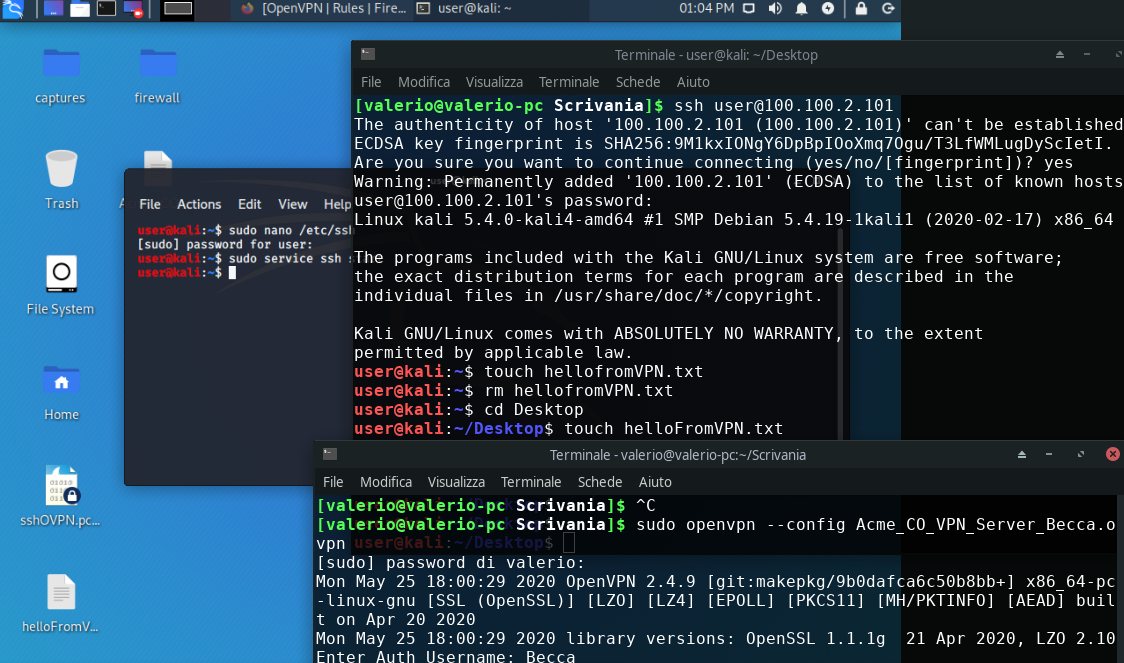
\includegraphics[width=1\textwidth]{OVPNaccessViaSSH.png}
  \caption[a]{User Becca accessing the Kali Machine via OpenVPN-SSH.}\label{fig:8}
\end{minipage}%
\end{figure}

\subsection{Testing the Proxy service}
We want the \textbf{squid proxy service} on the \textbf{proxy machine} to accept only users that have authenticated and are located in the \textbf{Clients subnetwork}, thus connections coming from a different subnetwork or the \textbf{WAN} are rejected a priori. In the \textbf{Kali machine}, we setup \textbf{Firefox browser} preferences so that it connects to the \textbf{proxy machine} requesting the \textbf{squid} service on port \textbf{3128} for every HTTP or HTTPS connection but those that have destination in the \textbf{Internal}, \textbf{External services} or \textbf{DMZ} subnetworks - \textit{manual configuration}. The figures below picture the desired behavior of both the services and the client's browser, which is now able to \textit{go out} in the \textbf{WAN} once the user is authenticated.\\

\begin{figure}[!htb]
\centering
\begin{minipage}{.5\textwidth}
  \centering
  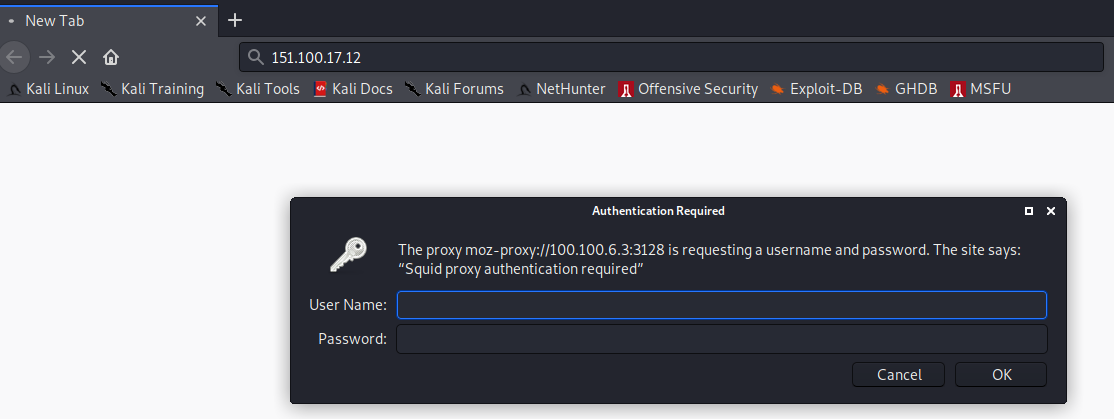
\includegraphics[width=1\textwidth]{proxyAuth.png}
  \caption[a]{Authentication procedure in the Kali machine's browser.}\label{fig:9}
\end{minipage}%
\begin{minipage}{.5\textwidth}
  \centering
  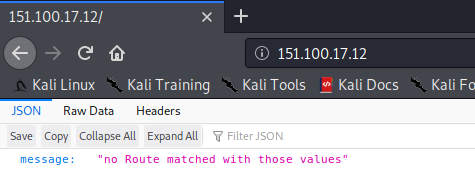
\includegraphics[width=1\textwidth]{proxyAuthed.png}
  \caption[a]{Successfully authenticated user can exploit proxy to display web pages outside of the network.}\label{fig:10}
\end{minipage}%
\end{figure}
